\documentclass[prb,aps,nobibnotes,twocolumn,doublespace,twocolumngrid,superbib]{revtex4}
%\documentclass[prb,aps,nobibnotes,superbib,preprint]{revtex4}

\usepackage{graphicx}
\usepackage{amsfonts}
\usepackage{amsmath}
\usepackage{bm}
\usepackage{alltt}
\usepackage{dcolumn} 
\usepackage{graphicx}
\makeatletter 
\makeatother 

\begin{document}

\title{An Exact Bounded Error Estimate for the Multipole Expansion}

\author{C. J. Tymczak}
\author{Matt Challacombe}

\affiliation{Theoretical Division, Los Alamos National Laboratory, Los Alamos,NM 87545, USA}

\date{\today}

\begin{abstract}
We derive an exact bounded error estimate for the multipole expansion in ${\cal R}^3$.
%
This expansion is used in many important algorithms such as the multipole tree-codes 
or the fast multipole method  algorithms. 
%
Examples include the large scale simulations of gravitationally bound systems, such as galaxies, to
the simulations of large charge distributions, such as di-polar proteins in water. 
%
Error control is essential in order to achieve both  accuracy and efficiency for these algorithms. 
%
Specifically, we then illustrate how this new exact multipole error bound can be incorporated 
into our existing  quantum chemical tree-code within the linear scaling {\bf MondoSCF} suite.
%  
We then illustrate, with several example systems,  how these modifications improves both the 
accuracy and efficiency of our quantum chemical tree code, where we have achieve orders of 
magnitude reduction of the computational cost.
%
\end{abstract}

\maketitle

\footnotetext[1]{\tt tymczak@lanl.gov}
\footnotetext[2]{\tt mchalla@lanl.gov}
\footnotetext[3]{\tt Preprint LA-UR-03-1948}


\section{INTRODUCTION}

%In many interesting and technically relevant areas it sometimes becomes essential to simulate 
%the behavior of large scale systems where the interaction 
%falls of as one over the distance. 
%
In the astrophysical simulation of the gravitational interaction, to the condensed matter simulations of 
electrostatic interactions, the interaction potential falls of as (where $\Delta_i$ is either the mass 
or the charge), 
\begin{equation}
\phi({\bf x})= \sum_i {\Delta_i \over |{\bf x} - {\bf x}_i|},
\end{equation}
% 
In both cases the interaction potential falls off with one over the distance, 
which leads to {\cal O}($N^2$) scaling with system size (a charge interacting with $N-1$ 
charges done $N$ times). 
%
Several algorithm's have been developed to overcome this limitation such as the 
Ewald Method (EM)  \cite{DFincham94} algorithm, 
Particle Mesh Ewald (PME) \cite{luty:94}  algorithm, 
the Fast Multipole Method (FMM) \cite{Singh93,shimada:94,singer:95a}  algorithm,
and the multipole tree-code (MTC) \cite{JSalmon94} algorithm. 
%
Of specific interest, and to illustrate our new error bound for the multipole expansion, 
are the multipole tree-code methods. 
%
Tree-codes have several important advantages over these other methods [ref]: i) 
they are easy to parallelize, ii) they allow easy and accurate calculation of the 
energies and the forces, iii) Periodic boundary conditions can be easily included [ref], iv) 
and, because of this work, they now have excellent error control compared to other methods.
%

Previous work on tree-code algorithm's has been severely limited by the lack of
a reasonable error estimate [ref]. 
%
This has severely hampered the utility of these methods, and to a large degree have negated the advantages
of tree-codes which we have stated above.
%
This is our main motivation for deriving our new error estimate because for quantum chemistry calculations, 
where the distributions weights can span several magnitudes, any problem with the multipole error 
estimate can lead to large uncontrollable error in the matrix elements. 
%
Which would usually force us to lower our error 
thresholds to unacceptable small levels, also increasing the time to compute the matrix by orders of
magnitude. 
%
This problem is easily rectified by our new bounded error estimate.
%
%
%

In the next section we first review the multipole expansion specifically to spherical multipoles [ref]. 
%
We then briefly review the multipole tree-code algorithm,and we then show how the efficiency of 
the multipole tree-code code is controlled by the efficiency of the error estimates. 
%
We then briefly outline the derivation of our exact error bound and how it can be easily implemented 
into existing codes which use the multipole expansion.
%
In the final section we illustrate how this exact error bound improves dramatically the efficiency 
and accuracy of our Quantum chemical tree code (QCTC) for quantum and classical simulations 
of di-polar water.


\section{The Multipole Expansion}

Consider figure {\ref{figure:MultInBox}}, where we have depicted $N$ distributions inside the bounded 
region $\Sigma$, and a interacting reference distribution, $a$. 
%
Here we are defining {\it distribution} as a confined area of charge, be it
a point charge or local function, such as a Gaussian.  
%
%Let us also consider the long range interaction to be electrostatic in nature.
%
A simple, but computationally expensive, method to calculated the 
interaction of distribution $a$ with all the distributions in the region $\Sigma$ is,
\begin{eqnarray}
V[\mathbf{R}_{a},\mathbf{R}_{\Sigma}] =
\sum_{i=1}^{N} \frac{\Delta_{a} \, \Delta_{i}}{|\mathbf{R}_{a}-\mathbf{R}_{i}|}
\end{eqnarray}
%
However, as mentioned above, this scales with the number of distributions in the box, 
leading to quadratic scaling for 
the total interaction energy of $N$ distributions. 
%
One solution to this poor scaling would be to calculate the multipoles (here we use 
spherical multipoles) of the set of distributions in the region $\Sigma$ at some center (in the 
figure depicted by the red cross hairs), and then interact the reference distribution $a$ with the 
multipoles via
%
\begin{eqnarray}
V[&&\mathbf{R}_{a}, \mathbf{R}_{\Sigma}]  = 
\frac{1}{2} \sum _{l=0}^{L}\, \sum _{l'=0}^{L'}\, \sum _{m=-l}^{l}\, 
\sum _{m'=-l'}^{l'}\, \nonumber\\
&& \left( -1\right) ^{l}
\, {\cal O}_{l}^{m}[\mathbf{R}_{a}]M_{l+l'}^{m+m'}[\mathbf{R}_{a}-\mathbf{R}_{\Sigma}]\, 
{\cal O}_{l'}^{m'}[\mathbf{R}_{\Sigma}]+\varepsilon \nonumber\\
\label{MultI}
\end{eqnarray}
%
where ${\cal O}_{l}^{m}[\mathbf{R}_{a}]$ is the spherical  multiple's of the distribution $a$, 
${\cal O}_{l'}^{m'}[\mathbf{R}_{\Sigma}]$ is the spherical  multiple's of the distributions in 
the region $\Sigma$,
$M_{l+l'}^{m+m'}[\mathbf{R}_{a}-\mathbf{R}_{\Sigma}]$ is the interaction tensor 
(see equations (A1-A3) in Appendix A), and $\varepsilon$ is the error we make by this approximation. 
In equation (\ref{MultI}) we have made use of the exact expansion [ref],
%
\begin{eqnarray}
&& \frac{1}{ {|\mathbf{R}-\mathbf{R'}}|}  = 
\frac{1}{2}\sum _{l=0}^{\infty}\, \sum _{l'=0}^{\infty}\, \sum _{m=-l}^{l}\, 
\sum _{m'=-l'}^{l'}\,\nonumber\\
&& \left( -1\right) ^{l} \,
{\cal \tilde O}_{l}^{m}[\mathbf{R}-\mathbf{P}]M_{l+l'}^{m+m'}[\mathbf{P}-\mathbf{Q}]\, 
{\cal \tilde O}_{l'}^{m'}[\mathbf{R'}-\mathbf{Q}]
\label{OneOverR}
\end{eqnarray}
%
given that $|\mathbf{R}-\mathbf{R'}| > |\mathbf{P}-\mathbf{Q}|$.

%
In our illustrative example, the  multipole tree code,  calculations ${\cal O}_{l}^{m}[\mathbf{R}_{a}]$ 
are usually of a particular angular momentum type, $l_0$, such that the sum over $L$ can be removed.
%
And also, the value of $L'$ are usually fixed at 
some maximum value, $L'=L_{max}$.
%
However, fixing the value of $L'$ creates the problem of how to control the accuracy of the calculation 
for the reference distribution $a$, which is of central importance if we want to have any hope of 
controlling our error.

%
% Figure 1
%
\begin{figure}
\caption{A set of $N$ distributions in a region $\Sigma$ and the interacting distribution $a$.
And we define ${\bf d}_{max}$ as the maximum distance of the distributions from the regions center.}
{\centering \includegraphics {MultInBox.ps} \par} 
\label{figure:MultInBox} 
\end{figure}

\section{Multipole Tree Codes}

One solution to this problem is presented in Figure {\ref{figure:TreeInBox}}. 
%
Instead of contracting the reference distribution $a$ with the multipole moments of all the 
distributions in the region $\Sigma$, which can lead to large errors, we contract our reference 
distributions with sub-regions of the original region such that our error is well controlled. 
%
The simplest method for achieving this is to split our original region into two sub-regions, then split 
these sub-regions int sub-sub-regions, etc. 
%
If we have $N$ distributions in the original region our splitting scheme gives us $N$ (sub)regions and, which 
we refer to as nodes on the {\bf tree}, 
and $N$ distributions, which we refer to as leafs of the {\bf tree}. 
%
This is also depicted in  Figure {\ref{figure:TreeInBox}}. 
%
So instead of contracting our reference distribution $a$ with the 
original region, we now contract it with the set of sub-regions, which should control the error. 
%
In general for our reference distribution we will need to visit {\cal O}($\log (N)$) nodes and 
leafs, which we also depicted in 
Figure {\ref{figure:TreeInBox}} . 
%
The only issue yet to be resolved is how we estimate the error due to the translations of the 
distributions multipoles to the (sub)regions centers; what should be our error criteria for whether 
or not we contract on this node, or recur down to the 
next two sub nodes of the {\bf tree}. 
%
In the next section we explore this issue.

%
% Figure 2
%
\begin{figure}
\caption{The regions and sub-regions that distribution $a$ interacts with, and the depiction of the
organization of the multipole of the {\bf tree}}
{\centering \includegraphics {TreeInBox.ps} \par} 
\label{figure:TreeInBox} 
\end{figure}

\section{Exact Error Bound of the Multipole Expansion} 

Several multipole error criteria have been devised for multipole tree codes [ref].
%
The simplest multipole error criteria which is most often used in applications is the, and
which we use as an illustration of the problems associated with using unbounded error estimates, is the 
{\it opening criteria}, which is due to Barn and Hut [ref],
\begin{equation}
\varepsilon_{oc} \approx \frac{ \left| {\bf d}_{max} \right| }{ \left| {\bf R}_a - {\bf R}_{\Sigma} \right|}
\label{OpenCri}
\end{equation} 
%
However, this suffers from several severe problems: 
\begin{itemize}
\item[i)] It does not take into account the decay of the multipoles
\item[ii)] It does not take into account the weight of the distributions within the region $\Sigma$, 
a serious problem for quantum chemistry codes where the distribution weights can span several orders 
of magnitude,
\item[iii)] It does not take into account the angular momentum type of the distributions,
\item[iv)] When $|R_a - R_{\Sigma}| \rightarrow |{\bf d}_{max}|$ it can significantly underestimate
the error.
\end{itemize}
%
To avoid this problem we have derived an exact bounded error estimate which significantly improves the 
performance of our multipole tree codes.
%
In Appendix A we give a complete derivation of this exact bounded error estimate for the translation of 
multipoles, here we just give a brief description. 
%
Let us start with the expression of the exact multipole error as,
\begin{eqnarray}
\label{MultErr}
\varepsilon \left( l_{0}\right) && =\bigg| \frac{1}{2}\sum _{l'=L_{max}+1}^{\infty }\, 
\sum _{m=-l_{0}}^{l_{0}}\, 
\sum _{m'=-l'}^{l'}\, \nonumber\\
&& \left( -1\right) ^{l}\, 
{\cal O}_{l_{0}}^{m}[\mathbf{R}_a]\, 
M_{l_{0}+l'}^{m+m'}
[{\mathbf{R}_a-\mathbf{R}_{\Sigma}}]\, {\cal O}_{l'}^{m'}[\mathbf{R}_{\Sigma}] \bigg| \nonumber\\
\end{eqnarray}
%
which are the multipoles that are not summed in equation (\ref{MultI}) 
(This is the same as equation (\ref{B7}) in Appendix A). What we then make use of is the
Uns{\"o}ld operator,
\begin{equation}
{\cal O}_{l}\left[ \left| \mathbf{R}\right| \right] =\sqrt{\sum _{m}(l-m)!(l+m)!
\left| {\cal O}_{l}^{m}
\left[ \mathbf{R}\right] \right|^{2}}
\end{equation}
Which we will refer to as the Uns{\"o}ld weight of the distributions in the region $\Sigma$. 
Using this definition allows us to rewrite the error bound as,
%
%
\begin{eqnarray}
\varepsilon \left( l_{0}\right) &&  \leq \frac{1}{2}\frac{{\cal O}_{l_{0}}\left[
\left| \mathbf{R}_a \right| 
\right] }{\left| \mathbf{R}_a-\mathbf{R}_{\Sigma}\right| ^{l_{0}+L_{max}+2}} \nonumber\\
&& \sum _{l=0}^{\infty }\frac{n\left[ 
l_{0},l+L_{max}+1\right] 
{\cal O}_{l+L_{max}+1}\left[\left| \mathbf{R}_{\Sigma} \right| \right] }{\left| \mathbf{R}_a-
\mathbf{R}_{\Sigma}\right| ^{l}}
\end{eqnarray}
%
%
where
\begin{equation}
n\left[ l,l'\right] =\sqrt{2} \frac{(l+l')!}{l!\, l'!}
\end{equation}
%
To continue with the main points of our derivation, we can then show that 
\begin{equation}
{\cal O}_{l}[\left| \mathbf{R}\right| ]\leq {\cal C} \left| \mathbf{d}_{max}\right| ^{l}
\label{Cbound}
\end{equation}
Where we refer to ${\cal C}$ as the asymptotic Uns{\"o}ld weight, is independent 
of $l$ and ${\bf d}_{max}$, and can be tabulated beforehand. 
Using equation (\ref{Cbound}) allows us to write our error bound in its final form
\begin{equation}
\varepsilon \left( l_{0}\right) \leq \frac{1}{2}\frac{{\cal C} \,{\cal O}_{l_{0}}\left[\left| 
\mathbf{R}_a\right| 
\right] \, n\left[ l_{0},L_{max}+1\right] \, \left| \mathbf{d}_{max}\right| ^{L_{max}+1}}{
\left| \left| 
\mathbf{R}_a-\mathbf{R}_{box}\right| -\left| \mathbf{d}_{max}\right| \right| ^{l_{0}+1}\left| \mathbf{R}_a-
\mathbf{R}_{box}
\right| ^{L_{max}+1}}
\end{equation}
This error bound solves all the problems associated with the {\it opening criteria} error estimate: 
\begin{itemize}
\item[i)] It takes into account the decay of the multipoles,
\item[ii)] It takes into account the weight of the distribution within the box,
\item[iii)] It takes into account the angular momentum type of the distributions,
\item[iv)] When $|R_a - R_{box}| \rightarrow |{\bf d}_{max}|$ it correctly bounds the error. 
\end{itemize}
%

For illustrative purposes, we can continue this analysis to include the multipole error made within the 
fast multipole algorithm, but in this case we are contracting distributions in two different regions. 
%
Making the assumption that $L=L'=L_{max}$ we can write the fast multipole error as
\begin{eqnarray}
&& \varepsilon_{FMM}   \leq  \nonumber\\
&& \frac{1}{2} \frac{{\cal C}_{\Sigma_1} {\cal C}_{\Sigma_2} 
\left| \mathbf{d}_{max}\right|^{L_{max}+1}}
{\left|\mathbf{R_{\Sigma_1}}-\mathbf{R_{\Sigma_2}}\right|^{L_{max}+1}
\left|\left|\mathbf{R}_{\Sigma_1}-\mathbf{R}_{\Sigma_2} \right|-\left| 
 \mathbf{d}_{max}\right| \right|}\nonumber\\
\label{FMM_EB}
\end{eqnarray}
where $|{\bf d}_{max}| = |{\bf d}_{max}^{\Sigma_1}|+|{\bf d}_{max}^{\Sigma_2}|$ and 
${\bf R}_{\Sigma_1}$ and ${\bf R}_{\Sigma_2}$ are the centers of, 
${\bf d}_{max}^{\Sigma_1}$ and ${\bf d}_{max}^{\Sigma_2}$ are maximum distance of 
the distributions from the centers, and
${\cal C}_{\Sigma_1}$ and ${\cal C}_{\Sigma_2}$ asymptotic Uns{\"o}ld weight of the distributions within 
region $\Sigma_1$ and region $\Sigma_2$.

\section{RESULTS}

\subsection{Illustration of the Exact Error Bound}

Figure \ref{figure:MultipoleErrorWaterC512} is a contour plot of the logarithm of the binned error for a 
classical di-polar water system of 512 molecule per unit cell 125 nearest neighbor cells for decreasing 
threshold $\tau$. 
%
We obtained this plot by transversing the tree. 
On each visited node on the tree, which is determined by whether our
bounded error estimated is less the $tau$, we calculated the actual actual error (y-axis), and then 
bin this number. 
%
The red  line is $\tau=Error$. If our bounded error estimate was incorrect, some distribution errors would
lie above the red line. 
%
As can be seen in this figure, no distribution error is ever above the red line, 
which shows that our bounded error estimate, at least for about one million nodes tests, is obeyed.
% 
Figure \ref{figure:MultipoleErrorWaterQ64} shows the same test as figure \ref{figure:MultipoleErrorWaterC512} 
except that it is a di-polar quantum water system with 64 molecules per unit cell and 
125 nearest neighbor cells. 
%
Again we see that no distribution error ever falls above the  $\tau=Error$, 
which is exceptional for the quantum system where the distributions weights can vary
many orders of magnitude, and where in this case approximately ten million nodes where tested.  

%
% Figure 3
%
\begin{figure}
\caption{A contour plot of the binned error calculated on each visited node of the multipole tree for a
classical water system of 512 molecules per unit cell with 125 image cells. 
The red line is the $\tau=Error$ line}
{\centering \includegraphics {Error_vs_TauMAC_bin_Water512.ps} \par} 
\label{figure:MultipoleErrorWaterC512} 
\end{figure}
%
% Figure 4
%
\begin{figure}
\caption{A contour plot of the binned error calculated on each visited node of the multipole tree for a 
quantum  water system of 64 molecules per unit cell with 125 image cells using the STO-3G basis set.
The red line is the $\tau=Error$ line}
{\centering \includegraphics{Error_vs_TauMAC_Water64_bin.ps} \par} 
\label{figure:MultipoleErrorWaterQ64} 
\end{figure}


\subsection{Scaling}

In Figure \ref{figure:TimeVsNwater} we show the time to calculate all the forces and the time it takes
to construct the tree, for increasing system size. 
%
The test system we used was classical water up to one quarter of a million molecules. 
%
A very important thing to note that at the  threshold level of $\tau=10^{-8}$, 
we could obtain significant speedup by increasing the maximum multipole expansion order. 
%
Since this effect has yet to be seen for the {\it opening criteria} error estimate, 
we decided to investigate further.
%
Figure \ref{figure:TimeVsTauWater4096} shows the timing results for 4096 classical water molecules 
per unit cell with 125 images for increasing threshold and maximum multipole expansion order. 
%
As can be seen for a large threshold that a low maximum expansion order was faster, but as 
the threshold was lowered, the larger expansion orders became faster, the
crossover happening around about $\tau=10^{-3}$. 
%
To our knowledge, this effect has yet to be observed and we attribute it to
the our bounded error estimate. 


%
% Figure 5
%
\begin{figure}
\caption{The time to both build the multipole tree, and calculate the force for every particle, for  
a classical water system with 125 image cells at a tolerance of $\tau=10^{-8}$ and $L_{max}=(4,6,8)$ 
for increasing system size.}
{\centering \includegraphics {Time_vs_N_water_2.ps} \par} 
\label{figure:TimeVsNwater} 
\end{figure}


%
% Figure 6
%
\begin{figure}
\caption{The time to calculate the force for a classical water system with 4096 molecules
per unit cell and 125 image cells for  decreasing tolerance and  $L_{max}=(4,5,6,7)$.}
{\centering \includegraphics {Time_vs_Tau_W4096.ps} \par} 
\label{figure:TimeVsTauWater4096} 
\end{figure}

\section{CONCLUSIONS}

We have presented a new exact bounded error estimate for the multipole approximation which 
is essential for the control of errors within several important algorithms such as the multipole tree-codes 
or the fast multipole method algorithms.
%
This is of significant importance for quantum chemistry codes because the distributions 
weights can span several orders of magnitude, but also this will have an impact on Astro-physical calculations
where a better bound on the calculation of the forces is needed. 
%
We have also shown that for classical and quantum simulations that our error bound, at least to 
about ten million tests, is obeyed. 
%
We then demonstrated that we achieve linear scaling for very large classical system, up to one million particles, 
when our new error bound is used. 
%
And finally, we have illustrated that we can achieve significant speedups
by increasing the multipole expansion order, at least for error tolerances 
$\tau < 10^{-3}$.

\section*{ACKNOWLEDGMENTS}

We would like to acknowledge Tommy Sewell and Ed Kober for there advise
and support. We would also like to thank Anders Niklasson for his help
in preparation of this manuscript. 

\bibliographystyle{apsrmp} 
\bibliography{mondo_new}


\appendix

\section{Derivation of the Exact Bounded Error Estimate}
Let us start by defining some useful quantities
\begin{equation}
\label{B1}
\widehat{O}_{l}^{m}\left[ \mathbf{R}\right] =\frac{\left| \mathbf{R}\right| ^{l}P_{l}^{m}
\left( \cos \theta _{\mathbf{R}}
\right) \, e^{-im\phi _{\mathbf{R}}}}{\left( l+m\right) !}\quad \; \; 
\end{equation}
%
\begin{equation}
\label{B2}
M_{l}^{m}\left[ \mathbf{R}\right] =\frac{\left( l-m\right) !\, P_{l}^{m}\left( \cos 
\theta _{\mathbf{R}}\right) \, 
e^{-im\phi _{\mathbf{R}}}}{\left| \mathbf{R}\right| ^{l+1}}
\end{equation}
\begin{equation}
\label{B3}
{\cal O}_{l}^{m}\left[ \rho ;\mathbf{P}\right] =\int _{V_{\infty }}\, d{\mathbf{r}}\, 
\widehat{O}_{l}^{m}\left[ 
{\mathbf{r}-\mathbf{P}}\right] \, \rho \left( \mathbf{r}\right) \qquad \; \; \; 
\end{equation}
Next, let us consider the expansion of the coulomb integral into the
multipole basis
%
\begin{eqnarray}
\int \, d{\mathbf{r}}\, d{\mathbf{r}'} \frac{\rho _{1}\left( \mathbf{r}\right) \: \rho _{2}
\left( \mathbf{r}'\right) }
{\left| \mathbf{r}-\mathbf{r}'\right| } \approx \frac{1}{2}\sum _{l=0}^{L}\, 
\sum _{l'=0}^{L'}\, \sum _{m=-l}^{l}\, 
\sum _{m'=-l'}^{l'}\qquad\nonumber\\
\left( -1\right) ^{l}{\cal O}_{l}^{m}[\rho _{1};\mathbf{P}]{M}_{l+l'}^{m+m'}[\mathbf{P}-\mathbf{Q}]\, 
{\cal O}_{l'}^{m'}[\rho _{2};\mathbf{Q}]\nonumber\\
\end{eqnarray}
%

\medskip\noindent{\bf MTC Error:} Let us now assume that the primitive 
distribution \( \rho _{1} \) is of a single angular momentum type and expanded about its center, 
%
\begin{equation}
\label{B5}
{\cal O}_{l}^{m}[\rho _{1};\mathbf{P}]={\cal O}_{l}^{m}[\rho _{1};\mathbf{P}]\delta _{l\, l_{0}}
\end{equation}
%
this gives us
%
\begin{eqnarray}
\int \, d{\mathbf{r}}\, d{\mathbf{r}'}\frac{\rho _{1}\left( \mathbf{r}\right) \: \rho _{2}
\left( \mathbf{r}'\right) }
{\left| \mathbf{r}-\mathbf{r}'\right| }
\approx \frac{1}{2}\sum _{l'=0}^{L'}\, \sum _{m=-l_{0}}^{l_{0}}\, 
\sum _{m'=-l'}^{l'}\, \qquad\nonumber\\
\left( -1\right) ^{l}\, {\cal O}_{l_{0}}^{m}[\rho _{1};\mathbf{P}]\, 
M_{l_{0}+l'}^{m+m'}[{\mathbf{P}-\mathbf{Q}}]\, 
{\cal O}_{l'}^{m'}[\rho _{2};
\mathbf{Q}] \nonumber\\
\label{B6}
\end{eqnarray}
%
The error in the calculation is then the multipoles that we do not sum
%
\begin{eqnarray}
\varepsilon \left( l_{0}\right) = \frac{1}{2}\sum _{l'=L'+1}^{\infty }\, 
\sum _{m=-l_{0}}^{l_{0}}\, 
\sum _{m'=-l'}^{l'}\qquad\qquad\qquad\nonumber\\ 
\left( -1\right) ^{l}
 {\cal O}_{l_{0}}^{m}[\rho _{1};\mathbf{P}]\, 
M_{l_{0}+l'}^{m+m'}
[{\mathbf{P}-\mathbf{Q}}]\, {\cal O}_{l'}^{m'}[\rho _{2};\mathbf{Q}]
\label{B7}
\end{eqnarray}
%
Let us define for the Uns{\"o}ld operator
%
\begin{eqnarray}
{\cal \widehat{O}}_{l}\left[ \left| \mathbf{P}\right| \right] &=& \sqrt{\sum _{m}(l-m)!(l+m)!
\left| \widehat{O}_{l}^{m}
\left[ \mathbf{P}\right] \right| ^{2}} \nonumber\\
&=&\left| \mathbf{P}\right| ^{l}\sqrt{\sum _{m}\frac{(l-m)!}{(l+m)!}
\left| P_{l}^{m}
(\mathbf{P})\right| ^{2}} \nonumber\\
&=& \left| \mathbf{P}\right| ^{l}\geq 0
\label{B8}
\end{eqnarray}
%
and similarly the Uns{\"o}ld weights
%
\begin{equation}
\label{B9}
{\cal O}_{l}[\rho ;\left| \mathbf{P}\right| ]=\sqrt{\sum _{m}(l-m)!(l+m)!\left| {\cal O}_{l}^{m}
\left[ \rho ;\left| 
\mathbf{P}\right| \right] \right| ^{2}}
\end{equation}
%
Let us rewrite the bounded error estimate as
%
\begin{eqnarray}
\varepsilon \left( l_{0}\right) \leq \frac{1}{2}\sum _{l'=L'+1}^{\infty } 
 \bigg|\sum _{m=-l_{0}}^{l_{0}}\, \sum _{m'=-l'}^{l'}
 \qquad\qquad\qquad\nonumber\\
{\cal O}_{l_{0}}^{m}[\rho _{1};\mathbf{P}]\, M_{l_{0}+l'}^{m+m'}
[{\mathbf{P}-\mathbf{Q}}]\, 
{\cal O}_{l'}^{m'}[\rho _{2};\mathbf{Q}]\bigg| \nonumber\\
\label{B10}
\end{eqnarray}
%
Let us also, for compactness of notation, define 
\begin{equation}
\label{B11}
{\cal O}_{l}^{m}\equiv {\cal O}_{l}^{m}[\rho _{1};\mathbf{P}]
\end{equation}
where the placement will indicate which distribution it is derived
from. Using equations (\ref{B2}) and (\ref{B3}) we can write this
as
%
\begin{eqnarray}
\varepsilon \left( l_{0}\right) \leq \frac{1}{2}\sum _{l'=L'+1}^{\infty } \bigg| 
\sum _{m=-l_{0}}^{l_{0}} \sum _{m'=-l'}^{l'} \qquad\qquad\qquad\qquad\qquad\nonumber\\
\frac{(l_{0}+l'-(m+m'))!  \,\, P_{l_{0}+l'}^{m+m'}\left( \cos \theta _{\mathbf{PQ}}\right)
}{\sqrt{(l_{0}+m)!(l_{0}-m)!}\: \sqrt{(l'+m')!(l'-m')!}}
\qquad\nonumber\\
\frac{\sqrt{(l_{0}+m)!(l_{0}-m)!}{\cal O}_{l_{0}}^{m} \, \sqrt{(l'+m')!(l'-m')!}
{\cal O}_{l'}^{m'}}{\left| \mathbf{P}-\mathbf{Q}
\right| ^{l'+l_{0}+1}}\bigg| \nonumber\\
\label{B12}
\end{eqnarray}
%
for reasons which will become apparent in what follows. Let us use
the inequalities (ref)
%
\begin{equation}
\label{B13}
\left| P_{l}^{m}\left( \cos \theta _{\mathbf{R}}\right) \right| \leq 1
\end{equation}
%
to simplify
%
\begin{eqnarray}
\varepsilon \left( l_{0}\right) \leq \frac{1}{2}\sum _{l'=L'+1}^{\infty }\, \bigg| 
\sum _{m=-l_{0}}^{l_{0}} \sum _{m'=-l'}^{l'} \qquad\qquad\qquad\qquad\qquad\nonumber\\
\frac{(l_{0}+l'-(m+m'))!}{\sqrt{(l_{0}+m)!(l_{0}-m)!}\: \sqrt{(l'+m')!(l'-m')!}} 
\qquad\nonumber\\
\frac{\sqrt{(l_{0}+m)!(l_{0}-m)!}\, {\cal O}_{l_{0}}^{m}
\sqrt{(l'+m')!(l'-m')!}\, 
{\cal O}_{l'}^{m'}}{\left| \mathbf{P}-\mathbf{Q}\right| ^{l'+l_{0}+1}}\bigg| \nonumber\\
\label{B14}
\end{eqnarray}
%
Now, let use the triangle inequality 
%
\[
\left| \mathbf{a}\cdot \mathbf{b}\right| \leq \left| \mathbf{a}\right| \left| \mathbf{b}\right| 
\qquad \qquad \]
\begin{equation}
\label{B15}
\left| \sum _{n}a_{n}\, b_{n}\right| \leq \sqrt{\sum _{n}\left| a_{n}\right| ^{2}\sum _{n'}
\left| b_{n'}\right| ^{2}}
\end{equation}
to get
%
%
%
\begin{eqnarray}
&& \varepsilon \left( l_{0}\right) \leq \frac{1}{2}\sum _{l'=L'+1}^{\infty } \nonumber\\
&& \qquad\bigg[ \sum _{m}^{l_0}  \sum _{m'}^{l'}
\frac{\left[ (l_{0}+l'-(m+m'))!\right] ^{2}}{(l_{0}+m)!(l_{0}-m)! (l'+m')!(l'-m')!} 
\nonumber\\
&& 
\qquad\sum_{m''}^{l_0} (l_{0}+m'')!(l_{0}-m'')!\left| {\cal O}_{l_{0}}^{m''}\right|^{2} \nonumber\\
&& 
\qquad\sum_{m'''}^{l'} (l'+m''')!(l'-m''')!\left| {\cal O}_{l'}^{m'''}\right| ^{2} \bigg]^{\frac{1}{2}}
\frac{1}
{\left|\mathbf{P}-\mathbf{Q}\right| ^{l'+l_{0}+1}}\nonumber
\end{eqnarray}
\begin{equation}
\label{B16}
\end{equation}
%
Which we can rewrite very compactly, using equation (\ref{B8}), as 
\begin{equation}
\label{B17}
\varepsilon \left( l_{0}\right) \leq \frac{1}{2}\sum _{l'=L'+1}^{\infty }\frac{{\cal O}_{l_{0}}
[\rho _{1};\left|
 \mathbf{P}\right| ]\: N\left[ l_{0},l'\right] \: {\cal O}_{l'}[\rho _{2};\left| \mathbf{Q}\right| ]}
{\left| 
\mathbf{P}-\mathbf{Q}\right| ^{l'+l_{0}+1}}
\end{equation}
where
\begin{equation}
N\left[ l,l'\right] =\sqrt{\sum _{m,m'}^{l_{0},l'}\frac{\left[ (l_{0}+l'-(m+m'))!
\right] ^{2}}{(l_{0}+m)!(l_{0}-m)! (l'+m')!(l'-m')!}}
\label{B18}
\end{equation}
However, we still have to eliminate the infinite sum over \( l' \)
within our error expression. Let us consider the limit of

\begin{equation}
\label{B19}
\lim _{l\rightarrow \infty }\left\{ {\cal O}_{l}[\rho ;\left| \mathbf{P}\right| ]\right\} ^{1/l}
\end{equation}
Considering the density as a sum of delta functions with arbitrary
weights. 
\begin{equation}
\label{B20}
\rho \left( \mathbf{r}\right) =\sum _{i}c_{i}\, \delta \left( \mathbf{r}-\mathbf{r}_{i}\right) 
\end{equation}
 then for the multipoles
%
\begin{equation}
\label{B21}
{\cal O}_{l}^{m}\left[ \rho ;\mathbf{P}\right] =\int _{V_{\infty }}\, d\mathbf{r}\, 
\widehat{O}_{l}^{m}\left[ 
\mathbf{r}-\mathbf{P}\right] \, \rho \left( \mathbf{r}\right) =\sum _{i}c_{i}\, 
\widehat{O}_{l}^{m}\left[ 
\mathbf{r}_{i}-\mathbf{P}\right] 
\end{equation}
%
and for the Uns{\"o}ld weights
%
\begin{eqnarray}
{\cal O}_{l}[\rho ;\left| \mathbf{P}\right| ] & = & \sqrt{\sum _{m}(l-m)!(l+m)!\left| 
{\cal O}_{l}^{m}\left[ 
\rho ;\left| \mathbf{P}\right| \right] \right| ^{2}} \nonumber\\
 & = & \sqrt{\sum _{m}(l-m)!(l+m)!\left| \sum _{i}c_{i}\, \widehat{O}_{l}^{m}\left[ 
\mathbf{r}_{i}-\mathbf{P}
\right] \right| ^{2}} \nonumber\\
\label{B22}
\end{eqnarray}
%
which we can rewrite using the addition theorem of angular momentum
as (ref)
%
\begin{equation}
\label{B23}
{\cal O}_{l}[\rho ;\left| \mathbf{P}\right| ]=\sqrt{\sum _{ij}c_{i}\, c_{j}^{*}\, \left| 
\mathbf{r}_{i}-
\mathbf{P}\right| ^{l}\left| \mathbf{r}_{j}-\mathbf{P}\right| ^{l}\, P_{l}\left[ 
\cos \gamma _{ij}\right] }
\end{equation}
which allows us to take the limit
\begin{equation}
\label{B24}
\lim _{l\rightarrow \infty }\left\{ {\cal O}_{l}[\rho ;\left| \mathbf{P}\right| ]\right\} ^{1/l}=
\lim _{l\rightarrow 
\infty }\left\{ \left| c_{I}\right| \, \left| \mathbf{d}_{max}\right| ^{l}\right\} ^{1/l}=\left|
 \mathbf{d}_{max}\right| 
\end{equation}
where \( \left| \mathbf{d}_{max}\right|  \)is the maximum distance
of a distribution to the contraction center \( \left| \mathbf{P}\right|  \).
Let us rewrite equation (\ref{B17}) as 
%
\begin{eqnarray}
\varepsilon \left( l_{0}\right) \leq \frac{1}{2}\frac{{\cal O}_{l_{0}}\left[ \rho _{1};\left|
 \mathbf{P}\right| 
\right] }{\left| \mathbf{P}-\mathbf{Q}\right| ^{l_{0}+L'+2}} 
\qquad\qquad\qquad\qquad\nonumber\\
\sum _{l=0}^{\infty }\frac{N\left[ 
l_{0},l+L'+1\right]
 {\cal O}_{l+L'+1}\left[ \rho _{1};\left| \mathbf{Q}\right| \right] }{\left| \mathbf{P}-\mathbf{Q}
\right| ^{l}} \nonumber\\
\label{B25}
\end{eqnarray}
%
Analyzing the behavior of \( N\left[ l,l'\right]  \) for large \( l' \)
we find that
%
\begin{eqnarray}
N\left[ l,l'\right] && \leq \alpha _{l}\frac{\left( \left( 1+l'\right) 
\left( 2+l'\right) \ldots \left( l+l'\right)\right) }{l!}\nonumber\\
&&=\alpha _{l}\frac{(l+l')!}{l!\, l'!}\equiv n\left[ l,l'\right] 
\label{B26}
\end{eqnarray}
%
where \( \alpha _{l}\leq \sqrt{2} \). Using equation (\ref{B26}), equation(\ref{B25})
can be written as
%
\begin{eqnarray}
\varepsilon \left( l_{0}\right) \leq \frac{1}{2}\frac{{\cal O}_{l_{0}}\left[ \rho _{1};\left| 
\mathbf{P}\right| \right] }{\left| \mathbf{P}-\mathbf{Q}\right| ^{l_{0}+L'+2}}
\qquad\qquad\qquad\qquad\nonumber\\
\sum _{l=0}^{\infty }\frac{n\left[ 
l_{0},l+L'+1\right] 
{\cal O}_{l+L'+1}\left[ \rho _{1};\left| \mathbf{Q}\right| \right] }{\left| \mathbf{P}-\mathbf{Q}
\right| ^{l}} \nonumber\\
\label{B27}
\end{eqnarray}
%
What remains is to determine the upper bound to \( {\cal O}_{l}\left[ \rho _{1};\left| 
\mathbf{Q}\right| \right]  \).
Analyzing equation (\ref{B23}) we can show that
\begin{equation}
\label{B28}
{\cal O}_{l}[\rho ;\left| \mathbf{P}\right| ]\leq C_{\rho }\left| \mathbf{d}_{max}\right| ^{l}
\end{equation}
Where \( C_{\rho } \) can be determined from
%
\begin{equation}
C_{\rho }\equiv \max_{l=L+1}^{\infty} \left( \frac{{\cal O}_{l}[\rho ;\left| \mathbf{P}\right| ]}{\left| 
\mathbf{d}_{max}\right|
 ^{l}}\right) 
\label{B28B}
\end{equation}
%
Using equation (\ref{B28}) the bounded error estimate can be rewritten as
%
\begin{eqnarray}
\varepsilon \left( l_{0}\right) && \leq \frac{1}{2}\frac{{\cal O}_{l_{0}}\left[ \rho _{1};\left| 
\mathbf{P}\right|
 \right] \, C_{\rho _{2}}\left| \mathbf{d}_{max}\right| ^{L'+1}}{\left| \mathbf{P}-\mathbf{Q}
\right| ^{l_{0}+L'+2}} \nonumber\\
&& \qquad\sum _{l=0}^{\infty }\frac{n\left[ l_{0},l+L'+1\right] \left| \mathbf{d}_{max}\right| ^{l}}{
\left| \mathbf{P}-
\mathbf{Q}\right| ^{l}}
\label{B29}
\end{eqnarray}
%
This can then be summed to the Hyper-geometric Function [ref]
%
\begin{eqnarray}
\varepsilon \left( l_{0}\right) && \leq \frac{1}{2}\frac{{\cal O}_{l_{0}}\left[ \rho _{1};\left| 
\mathbf{P}\right| 
\right] \, C_{\rho _{2}}\left| \mathbf{d}_{max}\right| ^{L'+1}}{\left| \mathbf{P}-\mathbf{Q}
\right| ^{l_{0}+L'+2}}n
\left[ l_{0},L'+1\right]\nonumber\\
&& \qquad { _{2}}F_{1}\left[ 1,\, l_{0}+L'+2,\, L'+2;\, \frac{\left| 
\mathbf{d}_{max}\right| }
{\left| \mathbf{P}-\mathbf{Q}\right| }\right]\nonumber\\
\label{B29B}
\end{eqnarray}
%
Which, to leading order can be simplified to
\begin{equation}
\label{B30}
\varepsilon \left( l_{0}\right) \leq \frac{1}{2}\frac{{\cal O}_{l_{0}}\left[ \rho _{1};\left| 
\mathbf{P}\right| 
\right] \, n\left[ l_{0},L'+1\right] \, C_{\rho _{2}}\left| \mathbf{d}_{max}\right| ^{L'+1}}{
\left| \left| 
\mathbf{P}-\mathbf{Q}\right| -\left| \mathbf{d}_{max}\right| \right| ^{l_{0}+1}\left| \mathbf{P}-
\mathbf{Q}
\right| ^{L'+1}}
\end{equation}
which bounds equation (\ref{B29B}).

\medskip\noindent{\bf FMM Error:}
We can also derive an bounded error estimate FMM methods. In the case of FMM methods, equation (\ref{B5}) 
does not apply, therefore our equations have to be modified. Starting with equation (\ref{B2}) we can 
show that the error bound can be written as
%
\begin{eqnarray}
\varepsilon_{FMM}  && \leq  
{\frac{1}{2}}\sum_{l=0}^{\infty} \sum _{l'=0}^{\infty }
\frac{{\cal O}_{l}[\rho _{1};\left|
\mathbf{P}\right| ]\: N\left[ l,l'\right] \: {\cal O}_{l'}[\rho _{2};\left| \mathbf{Q}\right| ]}
{\left| 
\mathbf{P}-\mathbf{Q}\right| ^{l+l'+1}} \nonumber\\
&&-{\frac{1}{2}}\sum_{l=0}^{L} \sum _{l'=0}^{L'}
\frac{{\cal O}_{l}[\rho _{1};\left|
\mathbf{P}\right| ]\: N\left[ l,l'\right] \: {\cal O}_{l'}[\rho _{2};\left| \mathbf{Q}\right| ]}
{\left| 
\mathbf{P}-\mathbf{Q}\right| ^{l+l'+1}} \nonumber\\
\label{B40}
\end{eqnarray}
%
Using equations (\ref{B26}) and (\ref{B28B}) we can rewrite this as
\begin{eqnarray}
\varepsilon_{FMM}  && \leq 
{\frac{C_{\rho_1} C_{\rho_2}}{2}} \bigg[
\sum_{l=0}^{\infty} \sum _{l'=0}^{\infty }
{\frac{\left| \mathbf{d} \right|^{l} n[l,l'] \left| \mathbf{d'} \right|^{l'}}
{\left|\mathbf{P}-\mathbf{Q}\right| ^{l+l'+1}}} \nonumber\\
&& \qquad\qquad\qquad-\sum _{l=0}^{L}\sum_{l'=0}^{L'}
{\frac{\left| \mathbf{d} \right|^{l} n[l,l'] \left| \mathbf{d'} \right|^{l'}}
{\left|\mathbf{P}-\mathbf{Q}\right| ^{l+l'+1}}} \bigg]\nonumber\\
\label{B41}
\end{eqnarray}
%where
%\begin{equation}
%C_{\rho }  \equiv   \max_{l=0}^{\infty} \left( \frac{{\cal O}_{l}[\rho ;\left| \mathbf{P}\right| ]}
%{\left| \mathbf{d}_{max}\right|^{l}}\right) 
%\label{B42}
%\end{equation}
This can be summed to get
%
\begin{eqnarray}
\varepsilon_{FMM} && \leq 
{\frac{C_{\rho_1} C_{\rho_2}}{2}} \bigg[ 
\frac{1}{\left|\left|\mathbf{P}-\mathbf{Q}\right|-\left| \mathbf{d} \right|-\left| \mathbf{d'} 
\right| \right|} \nonumber\\
&&\qquad\qquad\qquad-\sum _{l=0}^{L}\sum_{l'=0}^{L'}
{\frac{\left| \mathbf{d} \right|^{l} n[l,l'] \left| \mathbf{d'} \right|^{l'}}
{\left|\mathbf{P}-\mathbf{Q}\right| ^{l+l'+1}}} \bigg] \nonumber\\
\label{B43}
\end{eqnarray}
%
For the case where $L=L'$ this has a particularly simple form
\begin{equation}
\varepsilon_{FMM}  \leq \frac{1}{2}
\frac{ C_{\rho_1} C_{\rho_2} \left| |\mathbf{d}|+|\mathbf{d'}| \right|^{L+1}}
{\left|\mathbf{P}-\mathbf{Q}\right|^{L+1}
\left|\left|\mathbf{P}-\mathbf{Q}\right|-\left||\mathbf{d}|+|\mathbf{d'}|  \right|\right|}
\label{B44}
\end{equation}
\eject
\end{document}
